\documentclass{article}

\usepackage{standalone}

\begin{document}
    \textbf{Notation}: for the sake of 
    clarity, we will denote vectors
    as $\mathbf{x}$
    and their components as
    $x_{i}$ so that bold
    font identifies vectors
    and regular font
    indentifies real numbers. 
    
    \begin{exo}
    \end{exo} 
    Let $\mathcal{C}$ denote the set
    considered at each point in the exercise.
    \begin{itemize}
        \item The set $\mathcal{C}$ is the epigraph
            of the function
            $f \vcentcolon x \in \mathbb{R}
             \rightarrow \frac{1}{x}$.
             We have that $\dom f = \mathbb{R}_{+}^{*}$
             is convex and 
             $f''\left(x\right) = \frac{2}{x^{3}} \geq 0$
             for all $x \in \mathbb{R}_{+}^{*}$.
             Thus, \fbox{$\mathcal{C}$ is convex}.
         \item \fbox{The set $\mathcal{C}$ is
             not necessarily convex}.
             Indeed, let $e_{x} \defeq \left(x, 0, \ldots, 0\right)
             \in \mathbb{R}^{n}$ for
             any $x \in \mathbb{R}$.
             Let $S \defeq \left\{e_{-1},
             e_{1}\right\}$ and
             $T \defeq \left\{e_{0}\right\}$.
             We get that $e_{-1}, e_1 \in \mathcal{C}$
             but $\frac{1}{2} e_{-1} + \frac{1}{2} e_{1} = e_0
             \not\in \mathcal{C}$.
         \item We have that
             $x \in \mathcal{C}$ 
             if and only if
             for all $s_2 \in S_2$,
             there exists $s_1 \in S_1$
             such that $x = s_1 - s_2$.
             Thus, $\mathcal{C} = \bigcap_{
             s_2 \in S_2}
             S_{1} - s_2$. Since $S_1 - s_2$ 
             is convex for all $s_2 \in S_2$ 
             and the intersection
             of convex sets remains 
             convex, we get that
             \boxed{\text{the set $\mathcal{C}$ 
             is convex}}.
        \item Take $x_1, x_2 \in \mathcal{C}$.
            Thus, there exist
            $y_1, y_2 \in S_2$ 
            such that 
            $x_1 + y_1 \in S_1$ 
            and $x_2 + y_2 \in S_1$.
            For any $\alpha \in \left[0, 1\right]$,
            we have that
            $\alpha y_1 + \left(1 - \alpha\right)y_2
            \in S_2$ by convexity
            of $S_2$.
            Moreover, notice that
            \begin{equation}
                \label{S_1}
                \alpha x_1 + \left(1 - \alpha\right) x_2
                 + \alpha y_1 + \left(1 - \alpha\right) y_2 = 
                 \alpha\left(x_1 + y_1\right) +
                 \left(1 - \alpha\right)\left(x_2 + y_2\right).
            \end{equation}
            By convexity of $S_1$,
            the right-hand side of 
            (\ref{S_1}) is in $S_1$
            and so $\alpha x_1 + \left(1 - \alpha\right) x_2
            \in \mathcal{C}$.
            Thus \fbox{$\mathcal{C}$ is convex}.
     \end{itemize}

     \begin{exo}
     \end{exo}
     \begin{itemize}
         \item We compute the Hessian
             matrix $\Hess_{f}$.
             We have
             \begin{equation*}
                 \Hess_{f} = \begin{pmatrix}
                     0 & 1 \\
                     1 & 0
                 \end{pmatrix}.
             \end{equation*}
             We have that $\Hess_{f} \not \succeq 0$
             and $\Hess_{f} \not \preceq 0$.
             Therefore $f$ is not concave nor convex.
             Also, let $\alpha \in \mathbb{R}$.
             The set $S_{\alpha} \defeq
             \left\{\left(x_1, x_2\right) \in \mathbb{R}^{2} \mid x_1 x_2 \leq \alpha\right\}$ 
             is not covex nor concave.
             Therefore $f$ is not 
             quasiconvex nor quasiconcave.
         \item The Hessian matrix
             \begin{equation*}
                 \Hess_{f} = \begin{pmatrix}
                     0 & 1 \\
                     1 & 0
                 \end{pmatrix}
             \end{equation*}
             is such that $\mathbf{x}^{t} \Hess_{f} \mathbf{x} > 0$
             for all $x \in \mathbb{R}_{++}^{n}$.
             Since $\mathbb{R}_{++}^{n}$ is convex,
             we deduce that $f$ is convex
             (so it is also quasiconvex).
             By looking at $-\Hess_{f}$ we see
             that $f$ is not concave.
             Moreover, for any $\alpha \in \mathbb{R}$,
             the set $S_{\alpha}' \defeq 
             \left\{\left(x_1, x_2\right) \in \mathbb{R}^{2}_{++} 
             \mid - x_1 x_2 \leq \alpha\right\}$ 
             is convex for all $\alpha$.
             Therefore $f$ is quasiconcave.
         \item We have that
             \begin{equation*}
                 \Hess_{f}\left(x_1, x_2\right) = \begin{pmatrix}
                     0 & -\frac{1}{x_{2}^{2}} \\
                     -\frac{1}{x_{2}^{2}} & 2 \frac{x_1}{x_2^{3}}
                 \end{pmatrix}
             \end{equation*}
             and thus we compute
             \begin{equation}
                 \label{npd}
                 \begin{pmatrix}
                     y_1 & y_2
                 \end{pmatrix}
                 \begin{pmatrix}
                     0 & -\frac{1}{x_{2}^{2}} \\
                     -\frac{1}{x_{2}^{2}} & 2 \frac{x_1}{x_2^{3}}
                 \end{pmatrix}
                 \begin{pmatrix}
                     y_1 \\
                     y_2
                 \end{pmatrix}
                 = 
                 -2\frac{y_1y_2}{x_2^{2}}
                 +2 \frac{x_1y_2^{2}}{x_2^{3}}.
             \end{equation}
             For instance, the
             left-hand side of (\ref{npd})
             is positive for $y_1 = y_2 = 1$,
             $x_2 = 1$ and $x_1$ large enough.
             On the other hand,
             it is negative for $y_1 = y_2 = 1$,
             $x_2 = 1$ and $0 < x_1 < \varepsilon$ 
             for small enough.
             This entails that $\Hess_{f} \not \succeq 0 $
             and $\Hess_{f} \not \preceq 0$.
             Therefore $f$ is not
             convex nor concave.
             On the other hand, the set
             $S_{\alpha} = \left\{\left(x_1, x_2\right) \in \mathbb{R}_{++}^{n}
             \mid x_1/x_2 \leq \alpha\right\}
             = \left\{\left(x_1, x_2\right)
             \mid x_1 \leq \alpha x_2 \right\}$
             is a half-plane and
             so it is convex.
             Thus $f$ is quasiconvex.
             We show in the same
             way that $f$ is quasiconcave.
       \item Notice that $\mathbb{S}_{++}^{n}$ 
           is convex. Given this,
           it suffices to show that the
           function
           $g \vcentcolon 
           t \in \mathbb{R} \mapsto \Tr\left(A + tB\right)$, 
           is convex for
           all $A \in \mathbb{S}_{++}^{n}$
           and $B \in \mathbb{S}^{n}$
           at $t = 0$.
           Notice that,
           since $A \in \mathbb{S}_{++}^{n}$,
           $A$ is invertible and
           $A^{-1}B$ is symetric.
           Moreover, there exists
           $Q$ such that $A^{-1}B = Q \Lambda Q^{-1}$,
           where $\Lambda = \Diag\left(
           \lambda_{1}, \ldots,
           \lambda_{n}\right)$. 
           We also have that        
           $\left(I + t A^{-1}B\right) = 
           Q \left(I + t \Lambda\right)Q^{-1}$
           thus, for $t$ small
           enough, $I + t \Lambda$
           is invertible.
           Also, we remark that, 
           there exists
           $\widetilde{Q}$ such that
           $A = \widetilde{Q} \widetilde{\Lambda} \widetilde{Q}^{-1}$ 
           with $\widetilde{\Lambda} = 
           \Diag\left(\widetilde{\lambda}_{1},
           \ldots, \widetilde{\lambda}_{n}\right)$
           with $\widetilde{\lambda}_{i} > 0$ 
           for all $1 \leq i \leq n$.
           We thus have that 
           \begin{equation*}
               \left(A + tB\right)^{-1} = 
               \left(I + tA^{-1}B\right)A^{-1}
               Q \left(I  + t\Lambda\right)^{-1}Q^{-1}
               \widetilde{Q}^{-1} \widetilde{\Lambda} \widetilde{Q}.
           \end{equation*}
           Thus, $\Tr\left(\left(A + tB\right)^{-1}\right) = 
           \sum _{i = 1}^{n} \frac{1}{\widetilde{\lambda}_{i}
           \left(1 + t \lambda_{i}\right)}$. 
           We finally get
           $g''\left(t\right) = \sum_{i = 1}^{n}
           \frac{2\lambda_{i}^{2}}{\widetilde{\lambda}_{i}
           \left(1 + t \lambda_{i}\right)^{3}} > 0$ 
           for $t$ small enough.
           We finally get that
           $f$ is convex.
   \end{itemize}

   \begin{exo}
   \end{exo}
   \begin{itemize}
       \item For any $s \in \mathbb{R}^n$,
           let $h\left(\mathbf{x}\right) \defeq
           \mathbf{s}^t\mathbf{x} - \|\mathbf{x}\|^2_2$.
           By taking $\nabla h \left(
           \mathbf{x}\right) = s - 2x$, 
           we get $\nabla h\left(\mathbf{x_{*}}\right) = 0$ 
           iff $x_* = \frac{1}{2}\mathbf{s}$.
           Since $\mathbf{H}_{h} \preceq 0$,
           our choice of $x_*$ yields
           a maximum of $h$.
           Therefore,
           $\|\mathbf{s}\|_2^{2, *} = \frac{1}{2}\|\mathbf{s}\|_2^2
           - \frac{1}{4}\|\mathbf{s}\|_2^2
           = \frac{1}{4}\|\mathbf{s}\|^2_2$.
           
           For the $\ell_1$ norm, we observe the
           following.
           Let $s \in \mathbb{R}$. If $s > 0$,
           then we have that $\sup_{x \in \mathbb{R}}
           sx - \left|x\right| = +\infty$
           (by taking $x \rightarrow +\infty$ 
           if $s > 0$ and 
           $x \rightarrow -\infty$ 
           if $s < 0$).
           On the other hand,
           if $\left|s\right| \leq 1$,
           we have $sx - \left|x\right| \leq 0$,
           for all choices 
           of $x \in \mathbb{R}$.
           By chosing $x = 0$,
           we get that
           $sx - \left|x\right| = 0$.
           Now, let $\mathbf{s} \in \mathbb{R}^{n}$.
           If there exists $i_0$ 
           such that $\left|s_{i_0}\right| > 1$
           (that is, $\|\mathbf{s}\|_{\infty}
           > 1$), we deduce that,
           by choosing $x_{i} = 0$ 
           for all $i \neq i_0$
           and by letting $x_{i_0}$ 
           to infinity to with
           the appropriate sign,
           we obtain $\sup_{\mathbf{x} \in \mathbb{R}^{n}}
           \mathbf{s}^{t}\mathbf{x} - 
           \|\mathbf{x}\|_{1} = +\infty$.
           On the other hand,
           if $\|\mathbf{s}\|_{\infty} \leq 1$,
           we get that
           \begin{equation*}
               \sup_{\mathbf{x} \in \mathbb{R}^{n}}
               \mathbf{s}^{t}\mathbf{x}-
               \|\mathbf{x}\|_{1} =
               \sup_{\mathbf{x} \in \mathbb{R}^{n}}
               \sum_{i = 1}^{n}\left(
               s_{i}x_{i} - \left|x_{i}\right|
               \right) \leq 
               \sum_{i = 1}^{n}
               \sup_{x \in \mathbb{R}}
               \left(s_{i}x - \left|x\right|\right)
               \leq 0.
           \end{equation*}
           But such upperbound
           can be obtained by choosing
           $\mathbf{x} = \mathbf{0}$.

           All in all we have that
           $\|\cdot\|^{*}_{1} = \ind_{\left\{
           \|\cdot\|_{\infty} \leq 1\right\}}\left(\cdot\right)$
       \item Let $g * h$ denote the
           infimal convolution of $g$ and $h$.
           For any $\mathbf{s} \in \mathbb{R}^n$
           we have:
           \begin{align*}
               \left(g * h\right)^*\left(s\right) &=
               \sup_{\mathbf{x}} \mathbf{s}^t\mathbf{x}
               - \min_{\mathbf{u} + \mathbf{v} = \mathbf{x}}
               \left(g\left(\mathbf{u}\right) + h\left(\mathbf{v}\right)\right) \\
               &= \sup_{\mathbf{x}} \mathbf{s}^t\mathbf{x} + \max_{\mathbf{u} + \mathbf{v} = \mathbf{x}}
               \left(- g\left(\mathbf{u}\right) - h\left(\mathbf{v}\right)\right)\\
               &= \sup_{\mathbf{x}} \max_{\mathbf{u}+\mathbf{v}=\mathbf{x}}
               \left(\mathbf{s}^t\mathbf{x} - g\left(\mathbf{u}\right)
               -h\left(\mathbf{v}\right)\right) \\
               &= \sup_{\mathbf{x}} \max_{\mathbf{u}+\mathbf{v}=\mathbf{x}}
               \left(\mathbf{s}^t\mathbf{u} - g\left(\mathbf{u}\right)\right) + 
               \left(\mathbf{s^t}\mathbf{v} - h\left(\mathbf{v}\right)\right)\\
               &= \sup_{\mathbf{u}, \mathbf{v}} \left(
               \mathbf{s}^t\mathbf{u} - g\left(\mathbf{u}\right)
                 + \mathbf{s}^t\mathbf{v}
                 - h\left(\mathbf{v}\right)\right) \\
               &= \sup_{\mathbf{u}} \left(\mathbf{s}^t\mathbf{u} -g\left(\mathbf{u}\right)\right)
                +\sup_{\mathbf{u}} \left( \mathbf{s}^t\mathbf{v}
                - h\left(\mathbf{v}\right)\right).
           \end{align*}
           Thus, $\left(g *h\right)^*\left(\mathbf{s}\right)
           = g^*\left(\mathbf{s}\right) +
           h^*\left(\mathbf{s}\right)$.

           Now, we compute
           \begin{equation*}
               \min_{\mathbf{u} + \mathbf{v} = \mathbf{x}}
               \left(g\left(\mathbf{u}\right)
               + h\left(\mathbf{v}\right)\right)
               = \min_{\mathbf{u}+\mathbf{v} = \mathbf{x}}
               \left(\|\mathbf{u}\|_{1}
               + \frac{1}{2\alpha}\|\mathbf{v}\|_{2}^{2}\right)
               = \min_{\mathbf{u}}\left(\|\mathbf{u}\|_{1}
               + \frac{1}{2\alpha}\|\mathbf{x}
               - \mathbf{u}\|^{2}_{2}\right).
           \end{equation*}
           Let $h\left(\mathbf{u}\right)
           \defeq  \min_{\mathbf{u}}\left(\|\mathbf{u}\|_{1}
           + \frac{1}{2\alpha}\|\mathbf{x}
           - \mathbf{u}\|^{2}_{2}\right)$.
           We have:
           \begin{equation*}
               \min_{\mathbf{u}} h\left(\mathbf{u}\right)=
               \min_{\mathbf{u}}
               \left(\|\mathbf{u}\|_{1}
               + \frac{1}{2\alpha}\|\mathbf{u}\|_{2}^{2}\right)
               = \min_{\mathbf{u}}
               \left(
               \sum_{i=1}^{n} \left(
               \left|u_{i}\right| + 
               \frac{1}{2\alpha}
               \left(x_{i} - u_{i}\right)^{2}
               \right)
               \right) = 
               \sum_{i=1}^{n}
               \min_{u} \left|u\right| +
               \frac{1}{2\alpha} \left(x_{i} - u\right)^{2}.
           \end{equation*}
           Let $h_{i}\left(u\right) \defeq
           \left|u\right| + \frac{1}{2\alpha}
           \left(x_{i} - u\right)^{2}$.
           We compute the minimum of
           $h_{i}$ on $\mathbb{R} \setminus \left\{0\right\}$.
           We have that for anu $u \in \mathbb{R} \setminus \left\{0\right\}$,
           we get $h'_{i}\left(u\right) =
           \sgn\left(u\right) - \frac{1}{\alpha}
           \left(x_{i} - u\right)$.
           Also $h''_{i}\left(u\right) = \frac{1}{\alpha} > 0$.
           We first compute the minimum of $h_i$ on $\mathbb{R}_{-}^{*}$.
           We have:
           \begin{equation*}
               h'_{i} \left(u\right) = 0 \Longleftrightarrow 
               -1 + \frac{1}{\alpha} \left(x_{i} - u\right)=0
               \Longleftrightarrow u = x_{i} + \alpha.
           \end{equation*}
           Which requires $x_{i} + \alpha < 0$, i.e.
           $x_{i} < - \alpha$.
           
           We now compute the minimum of $h_{i}$ on
           $\mathbb{R}_{+}^{*}$.
           We have:
           \begin{equation*}
               h'_{i}\left(u\right) = 0 \Longleftrightarrow
               1 - \frac{1}{\alpha}\left(x_{i} - u\right) = 0
               \Longleftrightarrow u = x_{i} - \alpha.
           \end{equation*}
           Which requires $x_{i} > \alpha$.
           We thus have the existence of 
           a unique minimum of $h_{i}$ on
           $\mathbb{R} \setminus \left\{0\right\}$
           if either $x_{i} > \alpha$ or
           $x_{i} < - \alpha$.
           If such conditions are met, 
           we deduce that this is also
           a global minimum on $\mathbb{R}$ 
           by the continuity of $h_{i}$.

           Otherwise, if we have
           $-\alpha < x_{i} < \alpha$,
           we get $h'_{i}\left(u\right) < 0$ 
           for all $u < 0$ and
           $h'_{i}\left(u\right) > 0$ 
           for all $u > 0$.
           we deduce that, in such case,
           the minimum of $h_{i}$
           is attained at $0$.
           All in all, we have that
           \begin{equation*}
               m_{i} \defeq \min_{u} h_{i}\left(u\right)
               = 
               \begin{cases}
                   -x_{i} - \frac{1}{2}\alpha &\text{if } \hfill x_{i} < -\alpha, \\
                   \frac{x_{i}^{2}}{2 \alpha} &\text{if }\hfill -\alpha \leq x_{i} \leq \alpha, \\
                   x_{i} - \frac{1}{\alpha} &\text{if } \hfill x_{i} > \alpha.\\
               \end{cases}
           \end{equation*}
           And thus:
           \begin{equation*}
               f\left(\mathbf{x}\right) = 
               \min_{\mathbf{u}} h\left(\mathbf{u}\right) = 
               \sum_{i}^{n} m_{i}.
           \end{equation*}
           Finally we notice that since
           $f$ is continuous and $\dom\left(f\right) = \mathbb{R}^{n}$
           is closed, $f$ is a closed function.
           Moreover, since
           all the $m_{i}$s are convex,
           $f$ is also convex.
           Since $f$ is closed and
           convex,
           we have $f = f^{**}$.
       \item Let $f \vcentcolon x \in \mathbb{R} \mapsto 
           \log\left(1 + \exp\left(x\right)\right)$ and
           let $s \in \mathbb{R}$,
           we define $h \vcentcolon \mathbb{R} \rightarrow \mathbb{R}$
           by $h\left(x\right) = sx - \log\left(1 + \exp\left(x\right)\right)$.
           We have $h'\left(x\right) = s - \frac{\exp\left(x\right)}{1 + \exp\left(x\right)}$ 
           and $h''\left(x\right) = - \frac{\exp\left(x\right)}{\left(1 + \exp\left(x\right)\right)^{2}}<0$.
           So $h$ is concave.
           \begin{itemize}
               \item For $s < 0$, we have
                   $\lim_{x \rightarrow +\infty} h\left(x\right) = +\infty$.
               \item If $s = 0$, we have
                   $h\left(x\right) < 0$ and
                   $\lim_{x \rightarrow -\infty} h\left(x\right) = 0$.
               \item If $0 < s < 1$, we have
                   \begin{equation*}
                       h'\left(x\right) = 0 \Longleftrightarrow
                       s - \frac{\exp\left(x\right)}{1 + \exp\left(x\right)} = 0
                       \Longleftrightarrow
                       x = \log\left(\frac{s}{1 - s}\right).
                   \end{equation*}
                   By the concavity of $h$,
                   we have that 
                   \begin{equation*}
                       \sup_{x \in \mathbb{R}} h\left(x\right) =
                       s \log\left(\frac{s}{1-s}\right)
                       - \log\left(1 + \frac{s}{1-s}\right) =
                       s \log\left(s\right) + \left(1 - s\right) \log\left(1 - s\right).
                   \end{equation*}
               \item If $s = 1$, we have 
                   $h\left(x\right) = 
                   \log\left(\frac{\exp\left(x\right)}{1 + \exp\left(x\right)}\right) < 0$ 
                   and $\lim_{x \rightarrow +\infty} \log\left(\frac{\exp\left(x\right)}{
                   1 + \exp\left(x\right)}\right) = 0$.
              \item If $s > 1$, we have
                  $\lim_{x \rightarrow +\infty} h\left(x\right) = +\infty$.
           \end{itemize}
           All in all, we have that
           \begin{equation*}
               f^{*}\left(s\right) =
               \begin{cases}
                   +\infty &\text{if } \hfill s < 0,\\
                   0 &\text{if } \hfill s = 0,\\
                   s \log\left(s\right) + \left(1 - s\right)\log\left(1 - s\right)
                   &\text{if } \hfill 0 < s < 1,\\
                   0 &\text{if } \hfill s = 1,\\
                   +\infty &\text{if } \hfill s > 1.
               \end{cases}
           \end{equation*}
       \item The Lagrangian of \textsc{lasso} is
           \begin{equation*}
               \mathcal{L}\left(\mathbf{x}, \mathbf{y}, \mathbf{\lambda}\right) = 
               \frac{1}{2}\left\|\mathbf{y} - \mathbf{b}\right\|_{2}^{2} + 
               \alpha \left\|x\right\|_{1} +
               \mathbf{\lambda}^{t}\left(A\mathbf{x} - \mathbf{y}\right).
           \end{equation*}
           We exploit the fact that $\left(\alpha f\right)^{*}\left(\mathbf{s}\right)=
           \alpha f^{*}\left(\mathbf{s}/\alpha\right)$ 
           for all $\mathbf{s} \in \mathbb{R}^{n}$ and
           $\alpha \neq 0$ to deduce that
           $\left(\alpha\left\|\cdot\right\|_{1}\right)^{*} =
           \alpha \ind_{\left\{\left\|\cdot\right\|_{\infty} \leq 1\right\}}
           \left(\frac{\cdot}{\alpha}\right)=
           \ind_{\left\{\left\|\cdot\right\|_{\infty} \leq 1\right\}}
           \left(\frac{\cdot}{\alpha}\right)$.
           Similarly, we have
           $\left(\frac{1}{2}\left\|\cdot\right\|_{2}^{2}\right)^{*} = 
           \frac{1}{2}\left\|\cdot\right\|_{2}^{2}$.
           Finally we notice that
           $\left(f\left(\cdot - \mathbf{c}\right)\right)^{*} = 
           f^{*}\left(\cdot\right) + \left(\cdot\right)^{t}\mathbf{c}$.
           Therefore, we have that
           $\left(\frac{1}{2} \left\|\cdot - \mathbf{c}\right\|_{2}^{2}\right)^{*}
           \left(\mathbf{\lambda}\right)= 
           \frac{1}{2} \left\|\mathbf{\lambda}\right\|_{2}^{2}
           + \mathbf{\lambda}^{t}\mathbf{c}$.
           We finally get that the (Fenchel)
           dual for \textsc{lasso} is
           \begin{align*}
               & \max_{\mathbf{\lambda} \in \mathbb{R}^{m}}
               -\left(\frac{1}{2}\left\|\cdot\right\|_{2}^{2}\right)^{*}\left(\mathbf{\lambda}\right)
               -\left(\alpha\left\|\cdot\right\|_{1}\right)^{*}
               \left(-A^{t}\mathbf{\lambda}\right)\\
               = &\max_{\mathbf{\lambda}} -\frac{1}{2}
               \left\|\mathbf{\lambda}\right\|_{2}^{2}
               +\frac{1}{2}\left\|\mathbf{b}\right\|_{2}^{2}
               - \ind_{\left\{\left\|\cdot\right\|_{\infty} \leq 1\right\}}
               \left(-\frac{A^{t}\mathbf{\lambda}}{\alpha}\right)\\
               =& \max_{\mathbf{\lambda}} -\frac{1}{2}\left\|\mathbf{\lambda} + \mathbf{b}\right\|_{2}^{2}
               +\frac{1}{2}\left\|\mathbf{b}\right\|^{2}_{2}
               -\ind_{\left\{\left\|\cdot\right\|_{\infty} \leq 1\right\}}
               \left(-\frac{A^{t}\mathbf{\lambda}}{\alpha}\right)\\
               =& \max_{\mathbf{\lambda}} -\frac{1}{2}\left\|\mathbf{\lambda}-\mathbf{b}\right\|_{2}^{2}
               +\frac{1}{2}\left\|\mathbf{b}\right\|_{2}^{2}
               -\ind_{\left\{\left\|\cdot\right\|_{\infty} \leq 1\right\}}
               \left(\frac{A^{t}\mathbf{\lambda}}{\alpha}\right).
           \end{align*}
           Where the last equality is given
           by the change of variables
           $\mathbf{\lambda} \mapsto - \mathbf{\lambda}$.
           We have the desired result.
       \item To keep notation consistent, we denote
           by $\mathbf{w}^{\left(i\right)}$ what is
           denoted $w_{i}$ in
           the homework text. The
           $j$-th coordinate of $\mathbf{w}^{\left(i\right)}$ 
           will be denoted $\mathbf{w}^{\left(i\right)}_{j}$.
           It is clear that the original problem and
           the formulation with
           the intermediate 
           constraints are equivalent.
           The Lagrangian of the
           intermediate
           constrained problem is
           \begin{equation*}
               \mathcal{L}\left(\lambda, \nu, \mathbf{w}, \mathbf{w}^{\left(1\right)}, 
               \ldots, \mathbf{w}^{\left(m\right)}\right) =
               \frac{1}{m} \sum_{i = 1}^{m} h_{i}\left(\mathbf{w}^{\left(i\right)}\right)
               + \frac{\lambda}{2} \left\|\mathbf{w}\right\|^{2}_{2}
               + \sum_{i = 1}^{m}\nu_{i}^{t}\left(\mathbf{w}^{\left(i\right)} - \mathbf{w}\right).
           \end{equation*}
           We want to compute
           \begin{align*}
               g\left(\nu\right) &=
               \inf_{\substack{
               \mathbf{w} \in \mathbb{R}^{n} \\
               \mathbf{w}^{\left(1\right)}, \ldots, \mathbf{w}^{\left(m\right)} \in \mathbb{R}^{n}      
               }}
               \frac{1}{m} \sum_{i = 1}^{m} h_{i}\left(\mathbf{w}^{\left(i\right)}\right)
               + \frac{\lambda}{2} \left\|\mathbf{w}\right\|^{2}_{2}
               + \sum_{i = 1}^{m} \nu_{i}^{t} \left(\mathbf{w}^{\left(i\right)} - \mathbf{w}\right) \\
               &= \inf_{\substack{
               \mathbf{w} \in \mathbb{R}^{n} \\
               \mathbf{w}^{\left(1\right)}, \ldots, \mathbf{w}^{\left(m\right)} \in \mathbb{R}^{n}      
               }}
               \frac{1}{m} \sum_{i = 1}^{m}
               \left(
               h_{i}\left(\mathbf{w}^{\left(i\right)}\right) - \left(m \nu_{i}^{t}\right)\mathbf{w}^{\left(i\right)}
               \right)
               + \frac{\lambda}{2} \left\|\mathbf{w}\right\|_{2}^{2}
               - \sum_{i = 1}^{m} \nu_{i}^{t} \mathbf{w} \\
               &= - \frac{1}{m} \sum_{i = 1}^{m}
               \sup_{\mathbf{w}^{\left(i\right)} \in \mathbb{R}^{n}}
               \left(\left(m \nu_{i}^{t}\right)\mathbf{w}^{\left(i\right)} 
               - h_{i}\left(\mathbf{w}^{\left(i\right)}\right)\right)
               - \sup_{\mathbf{w} \in \mathbb{R}^{n}}
               - \frac{\lambda}{2} \left\|\mathbf{w}\right\|^{2}_{2}
               + \sum_{i = 1}^{m} \nu_{i}^{t}\mathbf{w}.
           \end{align*}
           We have that
           \begin{equation*}
               \sup_{\mathbf{w}^{\left(i\right)} \in \mathbb{R}^{n}}
               \left(\left(m \nu_{i}^{t}\right) \mathbf{w}^{\left(i\right)}
               - h_{i}\left(\mathbf{w}^{\left(i\right)}\right)\right)
               = h_{i}\left(m \nu_{i}\right)
           \end{equation*}
           Let $f \vcentcolon \mathbf{w} \in \mathbb{R}^{n}
           \mapsto - \frac{\lambda}{2} \left\|\mathbf{w}\right\|^{2}_{2}
           + \sum_{i = 1}^{m} \nu_{i} \mathbf{w}$.
           Notice that $f$ is concave.
           We have
           \begin{equation*}
               \nabla f \left(\mathbf{w}\right) =
               - \lambda \mathbf{w} + \sum_{i = 1}^{m} \nu_{i} = 0
               \Longleftrightarrow
               \mathbf{w} = \frac{1}{\lambda} \sum_{i = 1}^{m} \nu_{i}.
           \end{equation*}
           Finally:
           \begin{equation*}
               \sup_{\mathbf{w} \in \mathbb{R}^{n}}
               \sum_{i = 1}^{m} \nu_{i} \mathbf{w}
               - \frac{\lambda}{2} \left\|\mathbf{w}\right\|_{2}^{2} =
               \frac{1}{\lambda}
               \sum_{1 \leq i, j \leq m}
               \nu_{i}^{t} \nu_{j}
               - \frac{\lambda}{2}
               \left\|\frac{1}{\lambda}
               \sum_{i = 1}^{m} \nu_{i}
               \right\|_{2}^{2} =
               \frac{1}{2 \lambda}
               \left\|
               \sum_{i = 1}^{m} \nu_{i}
               \right\|_{2}^{2}.
           \end{equation*}
           All in all, we have:
           \begin{equation*}
               g\left(\nu\right) = 
               - \frac{1}{m} \sum_{i = 1}^{m}
               h^{*}_{i}\left(m \nu_{i}\right)
               - \frac{1}{2 \lambda} \left\|\sum_{i = 1}^{m} \nu_{i}\right\|_{2}^{2}.
           \end{equation*}

           Now, let $h_{i} \vcentcolon \mathbf{w} \in \mathbb{R}^{n}
           \mapsto \log\left(1 + \exp\left(
           -y_{i} \mathbf{x}_{i}^{t} \mathbf{w}\right)\right)$ 
           and denote
           $\ell \vcentcolon x \in \mathbb{R}
           \mapsto \log\left(1 + \exp\left(x\right)\right)$.
           We notice that 
           $\mathbf{w} \in \mathbb{R}^{n}
           \mapsto \exp\left(-y_{i} \mathbf{x}_{i}^{t} \mathbf{w}\right)$ 
           is concave and $\log$ is
           convex and non-decreasing.
           Thus, $h_{i}$ is convex.
           So, for any given $\mathbf{s} \in \mathbb{R}^{n}$,
           we get that the function
           $\varphi \vcentcolon 
           \mathbf{w} \in \mathbb{R}^{n}
           \mapsto \mathbf{s}^{t} \mathbf{w} - h_{i}\left(\mathbf{w}\right)$
           is concave.
           Set $x = -y_{i} \mathbf{x}_{i} \mathbf{w}$ 
           so that $\mathbf{w} = -\frac{y_{i} \mathbf{x}_{i}}{\left\|x_{i}\right\|_{2}^{2}}x$.
           For $s = -y_{i}\frac{\mathbf{s}^{t} \mathbf{x_{i}}}{\left\|\mathbf{x}_{i}\right\|_{2}^{2}}$ 
           we have:
           \begin{align*}
               &\sup_{x \in \mathbb{R}} - y_{i} \frac{\mathbf{s}^{t}\mathbf{x}_{i}}
               {\left\|\mathbf{x}_{i}\right\|_{2}^{2}}x - 
               \log\left(1 + \exp\left(
               -y_{i}\mathbf{x}_{i}^{t} \cdot
               \left(
               -\frac{y_{i} \mathbf{x}_{i}}{\left\|\mathbf{x}_{i}\right\|_{2}^{2}}x
               \right)
               \right)\right) =\\
               = &\sup_{x \in \mathbb{R}}
               sx - \log\left(1 + \exp\left(x\right)\right)
               = \ell^{*}\left(s\right)
               = \ell^{*}\left(-y_{i}
               \frac{\mathbf{s}^{t}\mathbf{x}_{i}}{\left\|\mathbf{x}_{i}\right\|_{2}^{2}}\right).
           \end{align*}
           All in all, we have that the Lagrangian dual to the
           logistic regression problem is
           \begin{equation*}
               g\left(\nu \right) = -\frac{1}{m} \sum_{i = 1}^{m} \ell^{*}\left(
               -y_{i}m\frac{\mathbf{\nu}_{i}^{t}\mathbf{x}_{i}}{\left\|\mathbf{x}_{i}\right\|_{2}^{2}}
               \right) -
               \frac{1}{2 \lambda} \left\|\sum_{i = 1}^{m} \nu_{i}\right\|_{2}^{2}.
           \end{equation*}
       \item We set th domain of this problem to be 
           $\mathbb{S}^{n}$. For any $X \in \mathbb{S}^{n}$,
           let $\left(\lambda_{i}\left(X\right)\right)_{i = 1}^{n}$ 
           be its eigenvalues enumerated
           with multiplicity.
           We claim that for any $X \in \mathbb{S}^{n}$,
           $\max_{Y \succeq 0} - \Tr\left(XY\right)$ 
           is finite iff $Y \succeq 0$.
           We have
           \begin{equation*}
               \max_{Y \succeq 0} - \Tr\left(XY\right) =
               \max_{Y \succeq 0} - \sum_{i = 1}^{n}
               \lambda_{i}\left(X\right) \lambda_{i}\left(Y\right) = 
               \begin{cases}
                   - \infty &\text{if } X \not \succeq 0, \\
                   0 &\text{otherwise}.
               \end{cases}
           \end{equation*}
           Indeed,if we have
           $X \not\succeq 0$, it has
           a strictly negative eigenvalue $\lambda_{i_{0}}$.
           Then, by taking $Y = \Diag\left(0, \ldots, 0, y, 0, \ldots, 0\right)$
           with $y$ at position $i_0$, we get
           $\Tr\left(XY\right) = -y \lambda_{i_0}$,
           which tends to $- \infty$
           for $y \rightarrow +\infty$.
           If $X \succeq 0$, then $-\Tr\left(XY\right) \leq 0$,
           so taking $Y = 0$ yields the 
           desired result.
           Therefore, the problem in the statement is
           equivalent to
           \begin{equation*}
               \min_{X \in \mathbb{S}^{n}}
               \max_{\substack{
               \lambda \in \mathbb{R}^{m} \\
               S \succeq 0
               }}
               \Tr\left(A_0X\right) +
               \sum_{i = 1}^{m}
               \lambda_{i}\left(\Tr\left(A_{i}X\right) - b_{i}\right)
               - \Tr\left(SX\right).
           \end{equation*}
           So, we can write the Lagrangian of the
           problem as
           \begin{equation*}
               \mathcal{L}\left(X, \lambda, S \right) = 
               \Tr\left(A_0X\right) +
               \sum_{i = 1}^{m} \lambda_{i}
               \left(\Tr\left(A_{i}X\right) - b_{i}\right) - 
               \Tr\left(SX\right).
           \end{equation*}
           We want to compute for $S \succeq 0$:
           \begin{align*}
               g\left(\lambda, S\right) &=
               \Tr\left(A_0X\right) +
               \sum_{i = 1}^{m}\lambda_{i}
               \left(\Tr\left(A_{i}X\right) - b_{i}\right) -
               \Tr\left(SX\right) \\
               &= \Tr\left(
               \left(
               A_0 + \sum_{i = 1}^{m} \lambda_{i}A_{i} -S
               \right)X
               \right)
               -\lambda^{t}\mathbf{b} \\
               &= 
               \begin{cases}
                   -\lambda^{t}\mathbf{b} &\text{if } 
                   A_0  + \sum_{i = 1}^{m}\lambda_{i}A_{i} - S = 0, \\
                   -\infty &\text{otherwise.}
               \end{cases}
           \end{align*}
           
           Notice that for $S_{*}$ to be optimal,
           we need to have $S_{*} = A_0 \sum_{i = 1}^{m} \lambda_{i}A_{i}$.
           If there exists an optimal $X_{*}$,
           then we have $-\Tr\left(S_{*}X_{*}\right) \leq 0$
           since $S_{*} \in \mathbb{S}^{n}$ and
           $\Tr\left(A_{i}X_{*}\right) - b_{i} = 0$
           for all $i$. This gives us primal feasibility.
           We also have $S \succeq 0$ by construction, which
           yields dual feasibility.
           Since $S_{*} = A_0 + \sum_{i = 1}^{m} \lambda_{i}A_{i}$,
           we have
           \begin{equation*}
               \frac{\partial \Tr\left(A_0X\right)}{\partial X} + 
               \sum_{i = 1}^{m} \frac{\partial \left(\Tr\left(A_{i}X\right) - b_{i}\right)}{\partial X} -
               \frac{\partial \Tr\left(S_{*}X\right)}{\partial X}
               = A_{0}^{t} + \sum_{i = 1}^{m}\lambda_{i} A_{i}^{t} - S_{*}^{t} = 0,
           \end{equation*}
           which yields the first order condition.
           Since our original problem is convex,
           having strong duality is equivalent
           to the missing KKT condition,
           which is complementary slackness,
           i.e. $-\Tr\left(S_{*}X_{*}\right) = 0$.
   \end{itemize}
   \begin{exo}          
   \end{exo}
   \begin{itemize}
       \item Let $p^{*}$ be the optimal
           value for the original formulation of the problem
           and let $q^{*}$ be optimal value
           for the reformulated version.
           Since a feasible solution of the
           original problem automatically gives
           a feasible solution to the
           reformulated problem (by setting
           $s_{i} = \max\left\{0, 1 - y_{i}\mathbf{x}_{i}^{t}\mathbf{w}\right\}$),
           we have $p^{*} \leq q^{*}$.
           Since minimizing the objective function 
           of the reformulated problem yields
           optimal $s_{i}^{*} = \max\left\{0, 1 - y_{i} \mathbf{x}_{i}^{t} \mathbf{w}^{*}\right\}$,
           we get that $q^{*} \leq p^{*}$.
           Therefore the two formulations are equivalent.

           The Lagrangian of the problem
           is the following:
           \begin{equation*}
               \mathcal{L}\left(\mathbf{w},\mathbf{s},\lambda, \lambda'\right) =
               \frac{1}{2}\left\|\mathbf{w}\right\|_{2}^{2}
               +\alpha \sum_{i = 1}^{m}s_{i}
               - \sum_{i =1}^{m}\lambda_{i}
               \left(\mathbf{w}^{t}\mathbf{x}_{i}y_{i} + s_{i} - 1\right)
               - \sum_{i = 1}^{m}\lambda'_{i} s_{i}.
           \end{equation*}
           Notice that the Lagrangian is convex in $\mathbf{w}$ 
           and $\mathbf{s}$.
           Thus, to compute the Lagrange dual, we compute
           \begin{equation*}
               \frac{\partial \mathcal{L}}{\partial \mathbf{w}} =
               \mathbf{w} - \sum_{i = 1}^{m}\lambda_{i}\mathbf{x}_{i}y_{i} = 0
               \Longleftrightarrow
               \mathbf{w} = X \lambda.
           \end{equation*}
           We also have
           \begin{equation*}
               \frac{\partial \mathcal{L}}{\partial \mathbf{s}}\Big|_{j}
               = \alpha - \lambda_{j} - \lambda'_{j} =0.
           \end{equation*}
           In order to achieve optimality we 
           need $\lambda_{i} \geq 0$ and
           $\lambda'_{i} \geq 0$,
           this implies that $\lambda_{j} \leq \alpha$.
           Therefore, plugging this into $\mathcal{L}$,
           we get
           \begin{align*}
               \mathcal{L}\left(\mathbf{w}^{*},
               \mathbf{s}^{*}, \lambda, \lambda'\right) &=
               \max_{\substack{0 \leq \lambda \leq \alpha \\ 0 \leq \lambda' \leq \alpha}}
               \left(
               \frac{1}{2}\left\|X \lambda\right\|_{2}^{2}
               - \sum_{i = 1}^{m} \lambda_{i}\left(\lambda^{t}X^{t}\right)\mathbf{x}_{i}y_{i}^{2}
               + \sum_{i = 1}^{m} \underbrace{\left(\alpha - \lambda_{i} - \lambda'_{i}\right)}_{=0}
               + \sum_{i = 1}^{m}\lambda_{i}
               \right) \\
               &= \max_{0 \leq \lambda \leq \alpha} \left(
               \frac{1}{2}\left\|X \lambda\right\|_{2}^{2} - 
               \lambda^{t} X^{t} X \lambda
               + \sum_{i = 1}^{m}\lambda_{i}
               \right) \\
               &= \max_{0 \leq \lambda \leq \alpha} D\left(\lambda\right).
           \end{align*}
           We note in passing that we have
           the natural estimate for $\mathbf{w} = X \lambda$.



       \item From now on, we will refer to the
           Projected Gradient Ascent algorithm
           as PGA and to the Randomized 
           Coordinate Ascent algorithm
           as RCA.

           We first prove that one iteration
           of (RCA) optimizes one
           dimension of $\lambda$ at a time.
           We first notice that we keep
           thoughout the algorithm the
           invariant $\mathbf{w}^{\left(k\right)} = X \lambda^{\left(k\right)}$,
           required for optimality of the primal variable.
           One iteration step
           consists in performing
           a gradient ascent step
           with respect to the randomly
           chosen variable $\lambda_{i_{k}}$.
           We have
           \begin{equation*}
               \frac{\partial D}{\partial \lambda_{i_{k}}} \left(\lambda\right) = 
               1 - y_{i_{k}} \mathbf{x}_{i_{k}}^{t}
               \left(\sum_{j = 1}^{m}y_{j}\mathbf{x}_{j} \lambda_{j}\right).
           \end{equation*}
           As for the step size, we choose a Newton-like
           step of $\left|\frac{\partial D}{\partial \lambda_{i_{k}}}\left(\lambda\right)\right|
           = \frac{1}{\left\|\mathbf{x}_{i_{k}}\right\|_{2}^{2}}$.
           The corresponding gradient ascent step is
           \begin{equation*}
              \lambda^{\left(k+1\right)}_{i_{k}} = 
              \lambda_{i_{k}}^{\left(k\right)} -
              \frac{1 - y_{i_{k}}\mathbf{x}_{i_{k}}^{t}\mathbf{w}^{\left(k\right)}}{\left\|\mathbf{x}_{i_{k}}\right\|^{2}_{2}}.
           \end{equation*}
           We project this onto $\left[0, \alpha\right]$ to ensure
           feasibility.

           We also keep our invariant $\mathbf{w}^{\left(k+1\right)} = X \lambda^{\left(k+1\right)}$.
           We only need to update the $i_{k}$-th dimension to get
           $\mathbf{w}^{\left(k + 1\right)} = \mathbf{w}^{\left(k\right)}
           + y_{i_{k}}\mathbf{x}_{i_{k}} \left(\lambda_{i_{k}}^{\left(k+1\right)} - \lambda_{i_{k}}\right)$.
           We have the desired result.
 
           Now, let us look at the performances of 
           these algorithms. One can look
           at and reproduce our same simulations
           at \url{https://github.com/vincenzo-politelli/CVX}.
           We tested the algorithms on the
           LIBSVM datasets ``sonar'' (208 samples 
           and 60 features).
           and ``mushrooms'' (8124 samples and
           112 features).
           For a value of $\alpha = 1$
           and a maximum number of iterations
           of $200$. We look at the primal-dual
           gap agains the number of
           iterations and we obtain the following.

           \begin{figure}[h!]
                \centering
                \begin{subfigure}{0.45\textwidth}
                    \centering
                    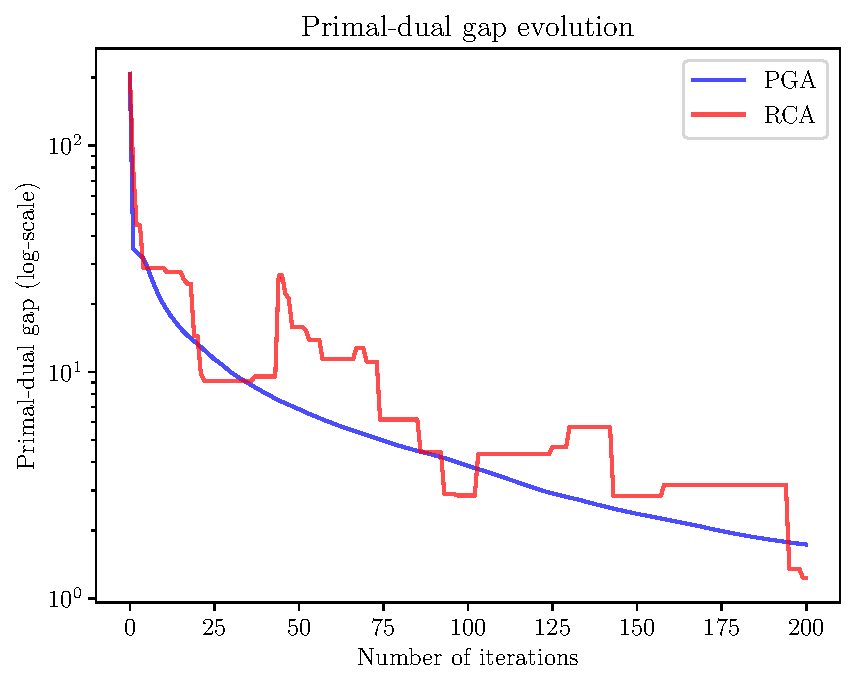
\includegraphics[width=\linewidth]{../code/plots/tiny_pd_plot.pdf}
                    \caption{Data for ``sonar'' dataset with $\alpha = 1$ and
                    a maximum number of iterations of $200$}
                    \label{pd_sonar}
                \end{subfigure}
                \hfill
                \begin{subfigure}{0.45\textwidth}
                    \centering
                    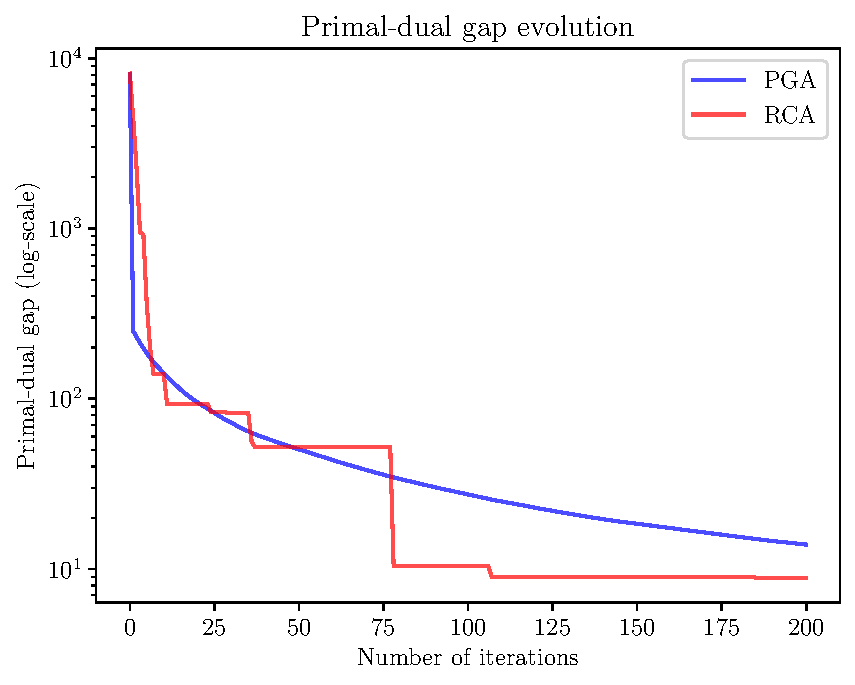
\includegraphics[width=\linewidth]{../code/plots/small_pd_plot.pdf}
                    \caption{Data for ``mushrooms'' dataset with $\alpha = 1$ and
                    a maximum number of iterations of $200$}
                    \label{pd_mushrooms}
                \end{subfigure}
                \label{fig:pd}
           \end{figure}
            
           We can see that the
           quality of the classification
           is comparable and that
           the primal-dual gap drops very quickly.
           In the case of the ``sonar'' dataset,
           for PGA, the final primal-dual gap is
           of $1.7312$; while in the case of
           RCA such value amounts to
           $1.2373$.
           In the case of the ``mushrooms''
           dataset, the primal-dual gap 
           for PGA is $13.9067$, while
           for RCA, such value is 
           $8.8974$. Thus, overall,
           RCA seems to be slightly more precise.
           We can see that the fact that 
           in RCA we do not take into account
           all the information about
           the gradient makes the convergence
           less smooth but still precise.
           On the other hand, RCA is much faster
           than PGA. Ineed, in the case
           of the ``sonar'' dataset,
           we PGA takes around $0.0164$ s to
           run, while RCA takes $0.0063$ s.
           In the case of the ``mushrooms''
           dataset, PGA takes $81.541$ s to 
           complete, while RCA takes only $0.1542$ s.
           We evince that the fact that
           RCA does not compute the whole
           gradient makes it much faster
           (but still precise enough).

           As for the misclassifications,
           we get that the two algorithms
           perform very well, the two
           dataset yielding $0$ misclassified
           samples only after the first few iterations.
           \newpage

           \begin{figure}[h!]
                \centering
                \begin{subfigure}{0.45\textwidth}
                    \centering
                    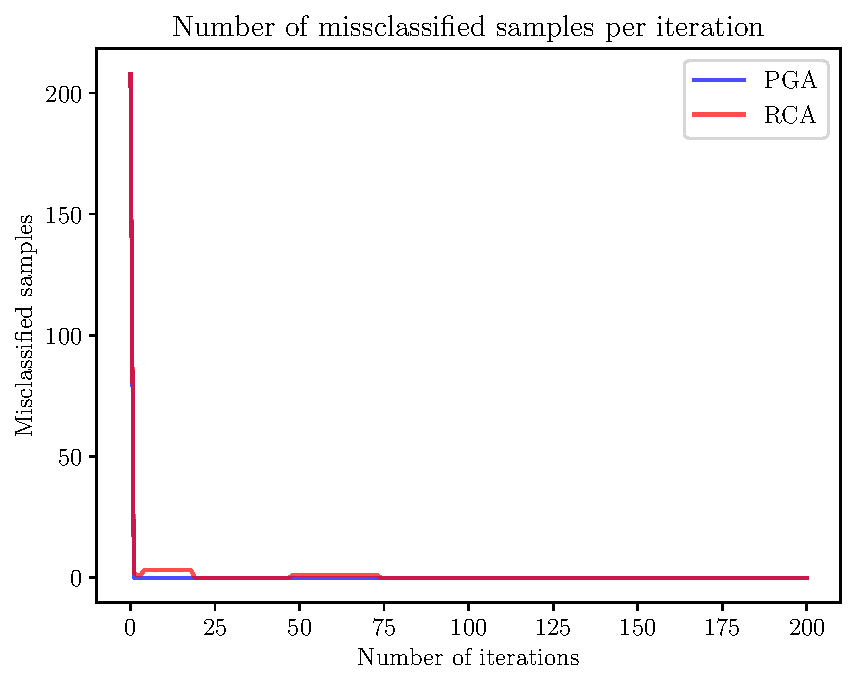
\includegraphics[width=\linewidth]{../code/plots/tiny_miss_plot.pdf}
                    \caption{Data for ``sonar'' dataset with $\alpha = 1$ and
                    a maximum number of iterations of $200$}
                    \label{miss_sonar}
                \end{subfigure}
                \hfill
                \begin{subfigure}{0.45\textwidth}
                    \centering
                    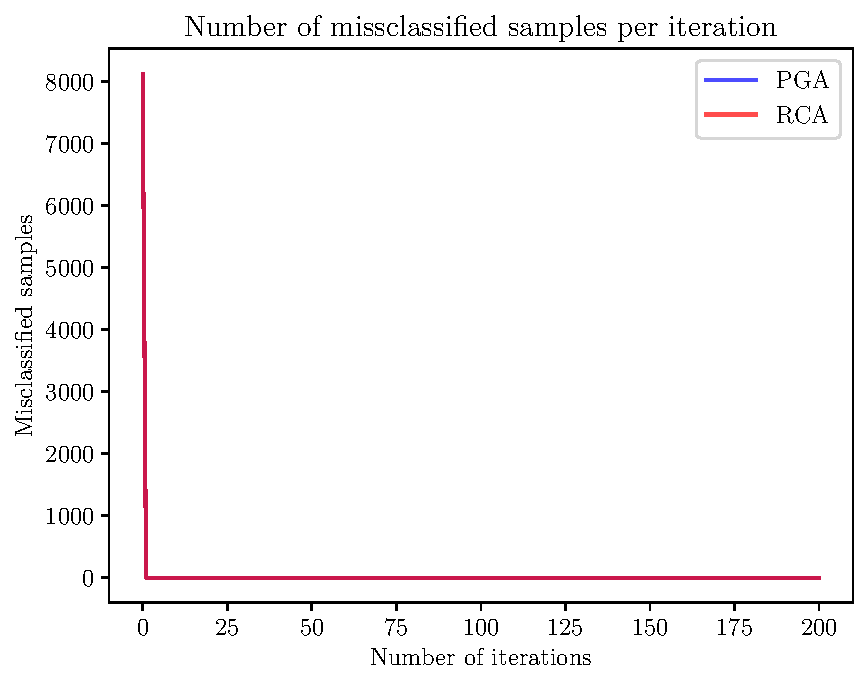
\includegraphics[width=\linewidth]{../code/plots/small_miss_plot.pdf}
                    \caption{Data for ``mushrooms'' dataset with $\alpha = 1$ and
                    a maximum number of iterations of $200$}
                    \label{miss_mushrooms}
                \end{subfigure}
                \label{fig:miss}
           \end{figure}

       \item Consider the LP problem
           \begin{align*}
               \min_{\substack{\mathbf{w}, \mathbf{v} \in \mathbb{R}^{n} \\
               \mathbf{v} \in \mathbb{R}^{m}}} \quad & 
               \sum_{i = 1}^{n}u_{i} + \alpha \sum_{i = 1}^{m}v_{i} \\
               \text{subject to} \quad & \mathbf{u} \geq \mathbf{w} \text{  and  } \mathbf{u} \geq -\mathbf{w}, \\
                                       & \mathbf{v} \geq \mathbf{0}_{n} \text{  and  } \mathbf{v} \geq \mathbf{1}_{n} - 
                                X^{t}\mathbf{w}.
           \end{align*}
           Let $p^{*}$ be the optimal solution
           to the original problem and let 
           $q^{*}$ bet the optimal solution to 
           the above reformulation. Clearly 
           any feasible solution to the original
           pr/oblem is a feasible solution
           of the reformulation.
           Thus  $p^{*} \leq q^{*}$.
           Moreover, since $w_{i} \geq \left|w_{i}\right|$
           and $v_{i} \geq \max \left\{0, 1 - y_{i}\mathbf{x}_{i}^{t}\mathbf{w}\right\}$,
           minimizing with respect to $\mathbf{w}, \mathbf{u}, \mathbf{v}$
           requires to choose $u_{i}^{*} = \left|w_{i}^{*}\right|$ 
           and $v_{i} = \max \left\{0, 1 - y_{i}\mathbf{x}_{i}^{t} \mathbf{w}^{*}\right\}$.
           Thus, $q^{*} \leq p^{*}$ and the two
           problems are equivalent.
           
           One can find on \url{https://github.com/vincenzo-politelli/CVX}
           the code that we use to solve this linear
           optimization problem. We have different
           values for the vector $\mathbf{w}$ (as 
           expected) and the method is 
           pretty fast, yielding an execution
           time of $0.01830$ s for the ``sonar''
           dataset and of $0.2853$ s for
           the ``mushrooms'' dataset.
           Thus, it seems to be just slightly less
           efficient than RCA.
           In this case as well, the final number
           of misclassified samples is $0$.

       \item We make the preliminary remark that
           feasible solutions to the above LP
           problem aways exist. Indeed
           if suffices to take $\mathbf{w} = \mathbf{1}_{n}$,
           $\mathbf{u} = \mathbf{0}_{n}$ and
           $v_{i} > \max\left\{0, 1 - y_{i}\mathbf{x}_{i}^{t}\mathbf{w}\right\}$ 
           for all $i$.
           Let $\mathbf{x}$ denote the concatenation
           $\left(\mathbf{w}, \mathbf{u}, \mathbf{v}\right)$ and 
           let $A$ be a matrix such that $A\mathbf{x} \leq 0$
           iff the linear constraints in the LP formulation
           above are satisfied. Let also
           $\mathbf{c} \defeq (
           \underbrace{0, \ldots, 0}_{\text{$n$-times}},
           \underbrace{1, \ldots, 1}_{\text{$n$-times}},
           \underbrace{\alpha, \ldots, \alpha}_{\text{$m$-times}})$.
           Let $n' \defeq 2n + m$. Then,
           we have the equivalent reformulation
           of the above LP problem.
           \begin{align*}
               \min_{\mathbf{x}} \quad & \mathbf{c}^{t}\mathbf{x} \\
               \text{subject to} \quad & A \mathbf{x} \leq 0 
           \end{align*}
           Let $A_{i}$ be the $i$-th row of
           $A$ and let $m'$ be the number of
           rows of $A$.
           As seen in the course, we consider
           the family of functions with
           logarithmic barrier which 
           are parametrized by $t > 0$:
           \begin{equation*}
               \varphi_{t} \vcentcolon \mathbf{x} \in \mathbb{R}^{n'}
               \mapsto t \mathbf{c}^{t}\mathbf{x}
               - \sum_{i = 1}^{m'} \log \left(A_{i}^{t}\mathbf{x}\right).
           \end{equation*}
           As seen in the course, we propose
           the following interior-point scheme (Algorithm \ref{algo}).
           \begin{algorithm}
               \label{algo}
               \caption{Interior-point method algorithm}
               \KwIn{A strictly feasible solution
               $\mathbf{x}$, $t = t_{0}>0$,
               $\varepsilon > 0$ and
               $\mu = 1 + 1/\sqrt{m'}$.}
               
               \SetKw{minimize}{minimize}
               \SetKw{quit}{quit}

               \While{True}{
                   \minimize $\varphi\left(t\right)$ by
                   Newton's method to get $\mathbf{x}^{*}\left(t\right)$\;
                   $\mathbf{x} \gets \mathbf{x}^{*}\left(t\right)$\;
                   \quit if $m'/t < \varepsilon$\;
                   $t \gets \mu t$\;
               }
           \end{algorithm}
           
           By the self-concordance of $\varphi_{t}$, 
           the analysis provided in the course
           yields that Newton's method
           takes at most $m'\left(\mu-1-\log\left(\mu\right)\right)$ 
           iterations to converge.
           We recall that one step of Newton's methods
           is of the form $\mathbf{x}^{+} = 
           \mathbf{x} - \nabla^{2}\varphi_{t}\left(\mathbf{x}\right)^{-1}
           \nabla \varphi_{t}\left(\mathbf{x}\right)$,
           and requires $\mathcal{O} \left(\left(n'\right)^{3}\right)$
           time.
           So, for $\mu = 1 + 1/\sqrt{m'}$, one iteration of our interior-point method
           algorithm takes time
           $m'\left(\frac{1}{\sqrt{m'}} - \log\left(1 + \frac{1}{\sqrt{m'}}\right)\right)
           \mathcal{O} \left(\left(n'\right)^{3}\right) =
           \mathcal{O} \left(\sqrt{m'} \left(n'\right)^{3}\right)$.
   \end{itemize}
 
\end{document}

